%!TEX root = cscw2018-comic.tex
\section{Motivating Ideas}
\label{sec:Motivating Ideas}
In this section, we present three key motivating ideas: social proof, information framing and abstract comics.

\subsection{Social Proof and Framing}
Two ideas ``social proof'' (from Psychology) and ``information framing'' (from Behavioral Economics) are central to our study. By ``social proof,'' we refer to the idea that individuals observing either their friends, or people with whom they can relate adopt a behavior, is persuasive for them to adopt the same behavior~\cite{Cialdini1993,Cialdini2004}. The use of ``social proof'' has been experimentally demonstrated in environmental conservation~\cite{goldstein2008room} and in energy conservation~\cite{schultz2007constructive}. Information framing refers to the idea that presenting outcomes as a gain or a loss, alters decisions~\cite{tversky1981framing,tversky1992advances}, since individuals are loss-averse and weigh losses more severely than similar gains.

% \begin{description}
%  % \item[Memorability] Approaches to make messages more persuasive has long been a focus for a variety of different fields including computational linguistics~\cite{danescu2012you} and advertising~\cite{Bradley2002,Chamblee1993,Knapp1981,Lowrey2006}. The most simple but effective way to achieve successful and long-last persuasion is through memorability.In \cite{danescu2012you} the study showed that using unusual word choices and more general theme makes it easier to connect with reader's daily life and makes the message more memorable. Through the use of unexpected words and phrases, the message is more likely to capture reader's attention compared text using normal phrases. But the theme should be as general as possible to help readers connect with the message, so it can stay in the reader's mind longer.
%  % Ford et. al \cite{ford1991memorability} looked into the memorability of messages in organ donation and suggests less typical arguments require higher cognitive loads to process and may result in internalizing the messages into pre-existing attitude which may affect behavior.

%  \item[Social Proof]: By ``social proof,'' we refer to the idea that individuals observing either their friends, or people with whom they can relate adopt a behavior, is persuasive for them to adopt the same behavior~\cite{Cialdini1993,Cialdini2004}.~\textcite{goldstein2008room} conducted an influential experiment in a hotel on motivating environmental conservation. They found that descriptive norms (e.g., ``the majority of guests reuse their towels'') has more persuasive power than solely mentioning environmental protection. And this normative message gets more effective when the statement is about a provincial norm (e.g., "the majority of guests in this room reuse their towels"). The work by~\textcite{schultz2007constructive} also demonstrated the effectiveness of the social norm in energy conservation. In a study of 300 households in San Marcos, California, the experimenters showed residents messages that compared their energy consumption to that of their neighbors. Surprisingly, there was no change in consumption---households below the mean increased consumption, while households above the mean decreased consumption. However, when households with above average energy consumption were shown the comparison along with a `frownie' face \frownie{}, and households with below average energy consumption were shown a `smiley' face \smiley{}, both groups' energy consumption decreased. This study illustrates the power of affect, but leads to the question of utility of the comic form for communication of more sophisticated affect.
%  \item[Information Framing]: ~\textcite{tversky1981framing,tversky1992advances} found that using different reference points to frame the same sentence can result in a different response. Consider the sentences ``there is a 50\% that you will be ill if you travel by plane to New York'' and ``there is a 50\% that you will be healthy if you travel by plane to New York.'' What~\textcite{tversky1981framing} showed is that  individuals have an asymmetric utility function weighting losses more severely than similar gains. Typically a gain has be twice as large as a loss to ``cancel'' out. In general, given two prospects, individuals favor risk seeking in when confronted with sure loss, and favor risk aversion when confronted with sure gain.
% \end{description}

% Since the prior work~\cite{goldstein2008room,schultz2007constructive} suggests a robust effect of the social proof, instead of using it as part of an experimental condition, we will incorporate it in the following way: we will have two characters in the comic, shown as friends. Second, we will show comparison of the individual to a group of friends. Thus our experimental condition tests the effect of information framing in comic form:

% \textbf{RQ}: \textit{What is the effect of information framing in modulating comic persuasiveness?}

\subsection{The Abstract Comic}
~\textcite{scott1993understanding} defines comics as ``juxtaposed pictorial and other images in deliberate sequence, intended to convey information and/or to produce an aesthetic response in the viewer." The simplicity of the comic form allows for delivering memorable messages~\cite{scott1993understanding}. In this study, we are motivated by the use of abstract comic form.~\textcite{scott1993understanding} points out that the reader is more likely to project themselves onto the character in the comic when the comic is more abstract. By taking the perspective of the character, the reader will internalize the information their character is trying to express or receive. If the information is persuasive, the internalization will imply a higher chance of target behavior change.~\Cref{fig:xkcd} shows an example.

% Beyond entertainment, comics can be used in scientific communication~\cite{McDermottPB18}, and for teaching in multilingual schools~\cite{cary2004going}.
% The simple and humorous nature of comic makes comics becomes an unique media for delivering informative and memorable messages. While reading comics book is commonly recognized as entertaining, comics have been examined as an effective way of communicating abstract ideas to broad audiences \cite{McDermottPB18,cary2004going,scott1993understanding}. McDermott et. al used comics to illustrate complex scientific facts \cite{McDermottPB18}. In education, comics have been used and examined as an effective tool for reaching different populations with various background \cite{McDermottPB18,cary2004going,scott1993understanding}.
% The use of metaphor in comics can make the underlying meaning vivid and more memorable than using a straightforward description \cite{McDermottPB18,scott1993understanding}. Moreover, comics can contain a personal story incredibly powerful for persuasion~\cite{weaver2017losing}. With a personal story, comics can create empathy for readers.~\textcite{matsubara2016emotional} showed a link between comic's content and the emotions felt by the readers. Thus complex messages can be easily interpreted and memorized though use of the comic form.



% Therefore, in this study, we choose to use an abstract yet well-recognized comic style, the xkcd style created by Randall Munroe~\cite{munroe2009xkcd}, in our generated persuasive comic messages; see~\Cref{fig:xkcd}. Thus a key research question is:

% \textbf{RQ}: \textit{Are statistical facts about individual behavior more persuasive when presented through abstract comic form?}

% \begin{figure}
%  \centering
%  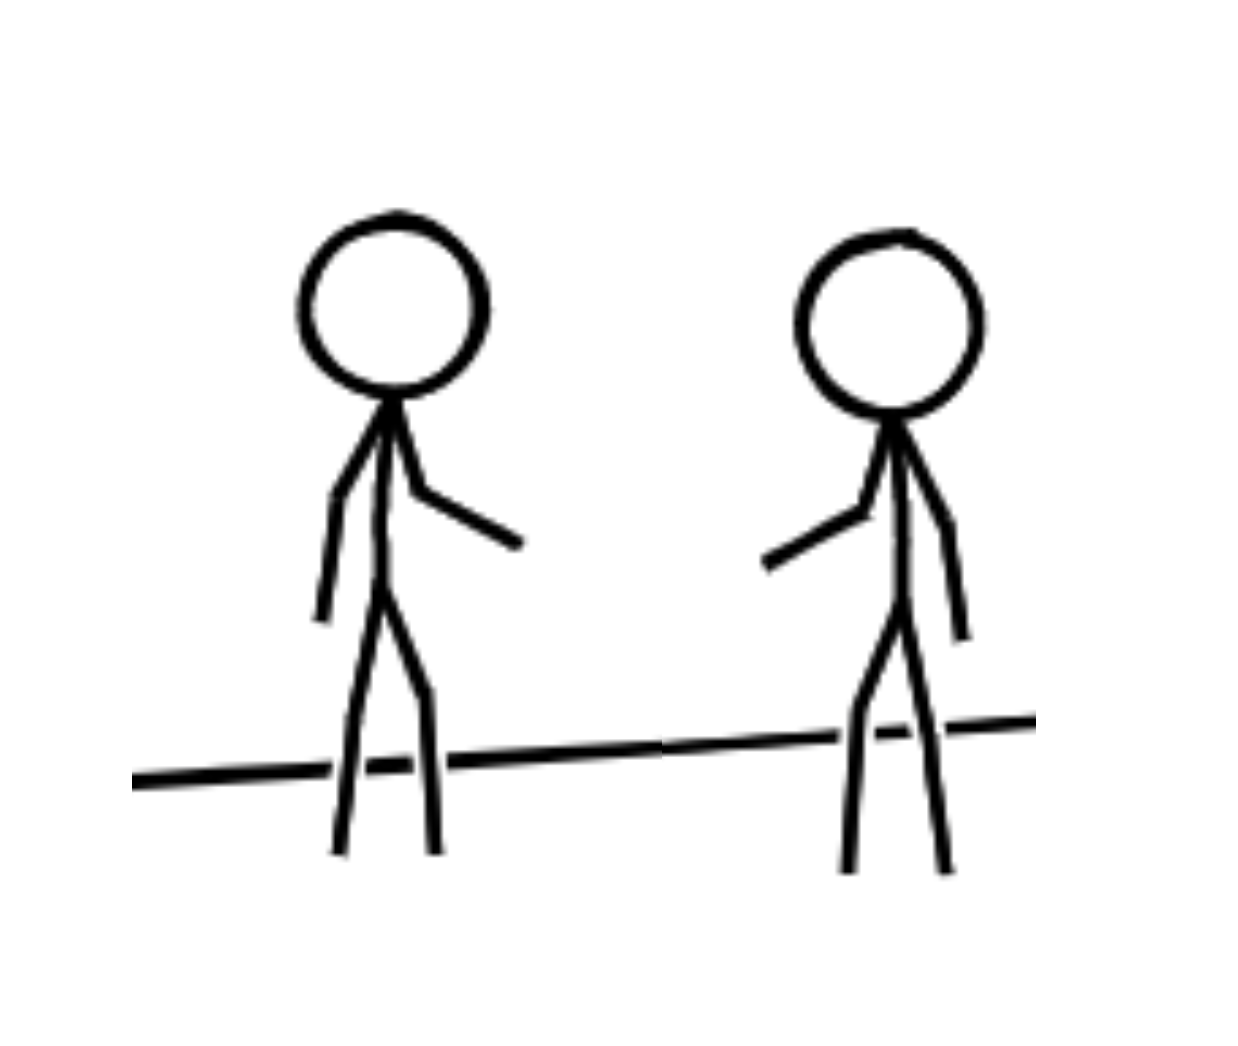
\includegraphics[width=0.3\columnwidth]{figures/xkcd_example}
%  \caption{A example of an abstract comic figure.}
%  \label{fig:xkcd}
% \end{figure}

\begin{wrapfigure}{R}{0.2\textwidth}
	\centering
	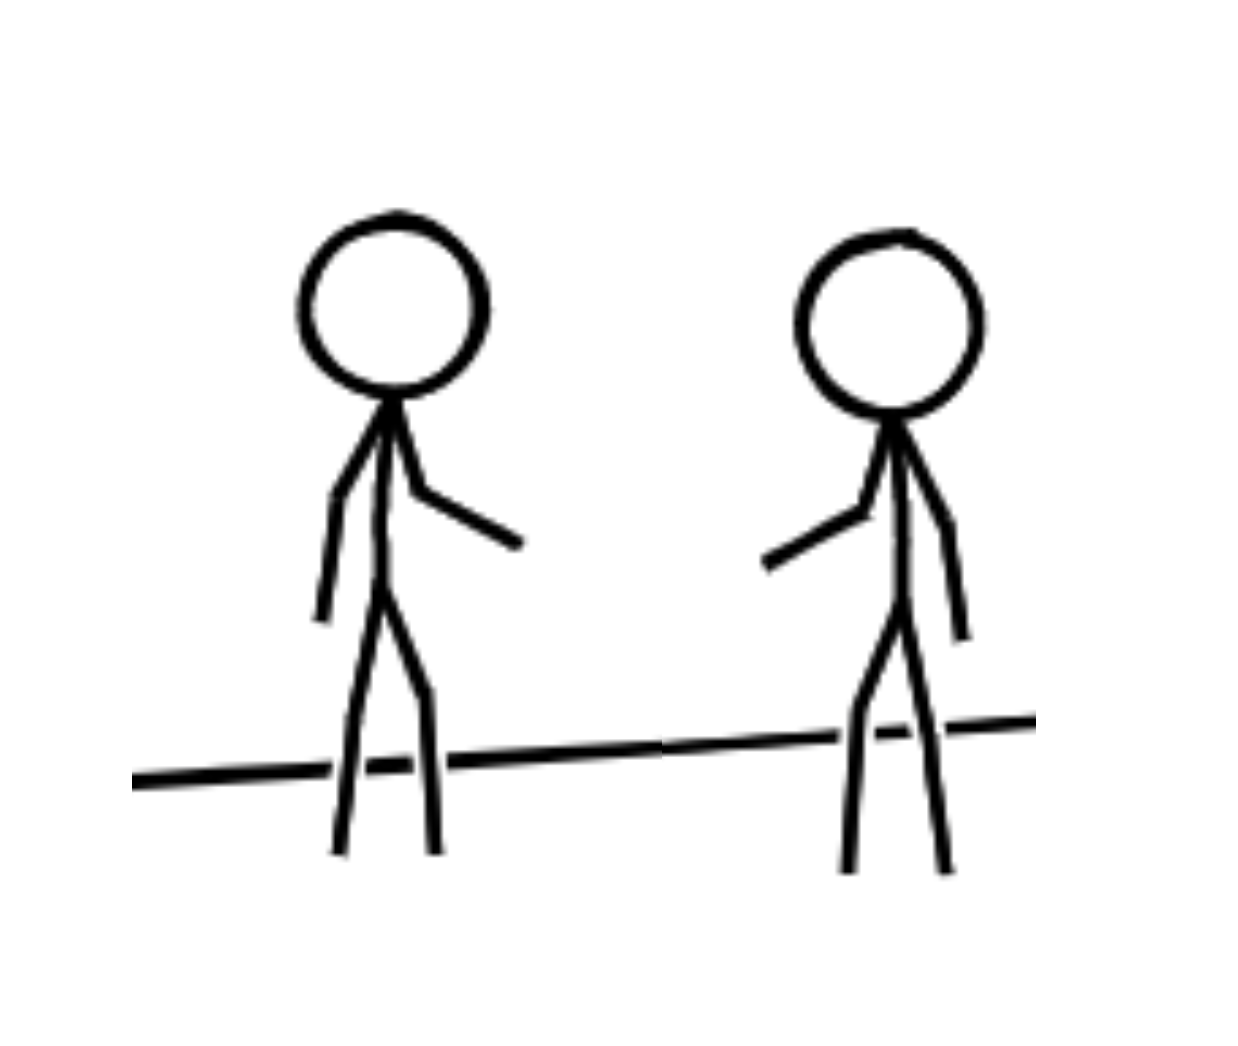
\includegraphics[width=0.19\textwidth]{figures/xkcd_example}
	\vspace{-10pt}
    \caption{An abstract comic example.}
    \label{fig:xkcd}
	\vspace{-10pt}
\end{wrapfigure}

~\textcite{scott1993understanding} identifies several fundamental components that influence reader reaction: character gestures, inter-character distance, and shading intensity. For example, the gesture of a character can help reader to understand interaction between characters and the emotion of the character. As a common technique, cartoonists often use the gesture to intensify the feeling that they want to communicate to the reader \cite{scott1993understanding}.
% In a persuasive message, the intensified emotion may make the message more memorable than a plain tone.
We plan to incorporate three variations of each of these elements in our first study.
% As a form of art, the creation of comics has few limitation. Although there is no common template that could describe all comics, if we take a closer look at each comic, it is not hard to see that every comic consists of several fundamental components. We categorize key comic elements into three groups: 1) character gestures, 2) inter-character distance, 3) background shading. To represent a persuasive message in comic form, we need to determine each of those three parameters.
% The gesture of a character is another important component in the comic.

% The relationship between characters is also important. Social proof suggests that messages are more persuasive if the person communicating the ideas is someone the receiver relates \cite{Cialdini1993}.
% In comics, the relationship between characters is modeled by the inter-character distance~\cite{scott1993understanding}.  A rich body of research has demonstrated the relationship between background shading and the emotion in comics~\cite{scott1993understanding}.

% The main research question:

% \textbf{RQ3}: \textit{What the effect of the elements of the comic form, specifically gesture, shading and distance between characters, in modulating comic persuasiveness?}
